\section{Inverted Files}
In order to speed up search of term occurrences, use indexing $\rightarrow$ \emph{Inverted files} is most widely used mechanism. It is appropriate when the text collection is \emph{semi-static}.

\paragraph{Definition} For a term $k$, \textbf{inverted list} $l_k = \langle f_k : d_{i_1}, ..., d_{i_{f_k}} \rangle$,

where $f_k$ is the $n^\circ$ of docs in which $k$ occurs, $d_{i_1}, ..., d_{i_{f_k}}$ is the list of identifiers of docs containing $k$.

\textbf{Inverted file} $IF = \langle i, k_i, l_{k_i}, i = 1,..., m \rangle$,

lexicographically ordered seq of inverted lists, constructed by concatenating the inverted lists \emph{of all terms occurring in the document collection}.

\paragraph{Example}Take the following document collection
\begin{lstlisting}
  B3 Automatic Differentiation of Algorithms: Theory, Implementation, and Application
  B5 Ideals, Varieties, and Algorithms: An Introduction to Computational Algebraic Geometry and Commutative Algebra
\end{lstlisting}

(Part of) The inverted file obtained is
\begin{lstlisting}
  1 Algorithms 2 : 3 5
  2 Application 1 : 3
  ...
\end{lstlisting}

\subsection{Physical organization}
Take into account quantitative characteristics $\longrightarrow$ \# references to docs (occurrences of index terms in docs) $\gg$ \# index terms (\# inverted lists). For a doc collection of size $n$
\begin{tabular}{ll}
  \textbf{\# occurrences of index terms}: & $O(n)$ \\
  \textbf{\# different index terms}: & $O(n^\beta)$
\end{tabular}

$\beta \approx 0.5$, according to Heap's law. So a doc collection of $10^6$ entries would have approx. $10^3$ index terms.

\paragraph{In main memory} Store \textbf{index terms} and \textbf{frequencies of occurrences} in index file. Access typically by \emph{binary search}, \emph{hash tables}, \emph{B+-Trees}, \emph{tries}.
\paragraph{In secondary storage} Store \textbf{posting file} and \textbf{document file}, where the posting file is a document that stores the occurrence of a term in a document in the collection. For each \emph{index term} $\longrightarrow$ relevant start position in \emph{posting file}. Occurrences in \emph{posting file} $\longrightarrow$ entries in \emph{document file}.

\subsection{Searching the Inverted File}

\begin{figure}
  \centering
  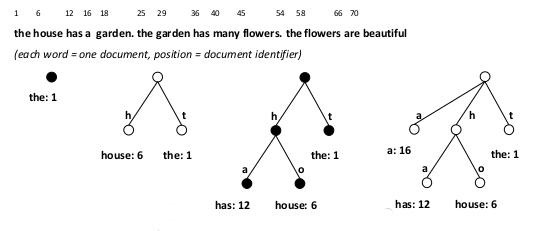
\includegraphics[width=\linewidth]{figures/trie_vocabulary.png}
  \caption{Construction of the trie structure for a given text}
  \label{fig:trie_vocabulary}
\end{figure}

\begin{description}

  \item[Vocabulary search]
  \begin{itemize}
    \item[]
    \item Vocabulary kept in \emph{trie} (\cref{fig:trie_vocabulary})
    \item Word $\longrightarrow$ list of occurrences
    \item Read text sequentially, search in vocabulary
    \item If not found, add to vocabulary with empty list
    \item Add word position to end of list
  \end{itemize}

  \item[Retrieval of occurrences] (from posting file) after complete traversal $\rightarrow$ cost $O(n)$
  \begin{itemize}
    \item Write list of occurrences contiguously to \emph{posting file} (\cref{fig:trie_to_postings})
    \item Use trie structure as data access for index in main memory
  \end{itemize}

  \item[Manipulation of occurrences] (e.g. compute term frequencies)

\end{description}

\begin{figure}
  \centering
  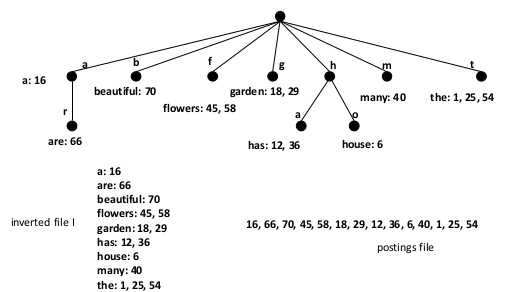
\includegraphics[width=\linewidth]{figures/trie_to_postings.png}
  \caption{Derive inverted file \& postings file from trie structure. Traverse top-down and left-to-right. Add new index terms to end of inverted file (occurrence to postings file).}
  \label{fig:trie_to_postings}
\end{figure}
